\documentclass[border=4pt]{standalone}
\usepackage[T1]{fontenc}
\usepackage{newtxtext,newtxmath}
\usepackage{tikz}
\usetikzlibrary{arrows.meta,calc,positioning}
\definecolor{ink}{HTML}{24313E}
\definecolor{blue}{HTML}{4477AA}
\definecolor{teal}{HTML}{338899}
\definecolor{amber}{HTML}{BB7711}
\definecolor{red}{HTML}{AA4455}
\begin{document}
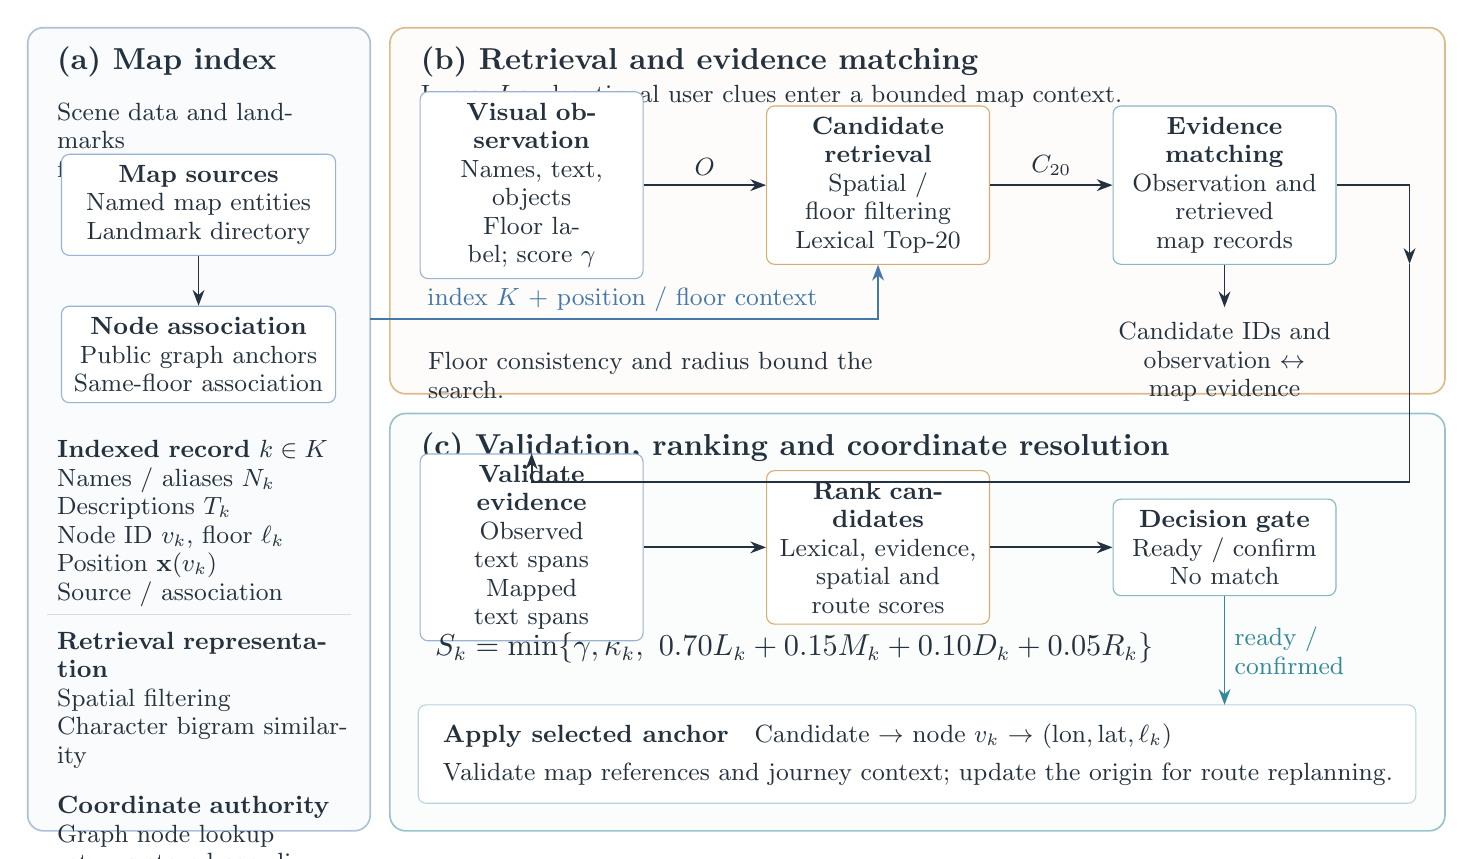
\begin{tikzpicture}[x=1cm,y=-1cm,text=ink,
 font=\fontsize{9}{10.5}\selectfont,
 arr/.style={-{Stealth[length=2mm]},line width=.65pt,draw=ink},
 panel/.style={rounded corners=2mm,line width=.6pt},
 box/.style={draw=blue!55,fill=white,rounded corners=1mm,align=center,font=\fontsize{8.7}{10.3}\selectfont,minimum height=1cm,text width=2.8cm,inner sep=4pt},
 smalltext/.style={font=\fontsize{8.7}{10.3}\selectfont,align=left},
 title/.style={font=\fontsize{11}{13}\selectfont\bfseries,anchor=west}]
\path[use as bounding box] (0,0) rectangle (18,10.2);
\draw[panel,draw=blue!45,fill=blue!3] (0,0) rectangle (4.35,10.2);
\draw[panel,draw=amber!50,fill=amber!2] (4.6,0) rectangle (18,4.65);
\draw[panel,draw=teal!50,fill=teal!2] (4.6,4.9) rectangle (18,10.2);
\node[title] at (.25,.43) {(a) Map index};
\node[smalltext,anchor=north west,text width=3.75cm] at (.25,.83)
 {Scene data and landmarks\\form structured records.};
\node[box,text width=3.2cm] (src) at (2.17,2.25)
 {\textbf{Map sources}\\Named map entities\\Landmark directory};
\node[box,text width=3.2cm] (attach) at (2.17,4.15)
 {\textbf{Node association}\\Public graph anchors\\Same-floor association};
\draw[arr] (src)--(attach);
\node[smalltext,anchor=north west,text width=3.75cm] at (.25,5.12)
 {\textbf{Indexed record $k\in K$}\\Names / aliases $N_k$\\Descriptions $T_k$\\Node ID $v_k$, floor $\ell_k$\\Position $\mathbf{x}(v_k)$\\Source / association};
\draw[blue!25] (.25,7.45)--(4.1,7.45);
\node[smalltext,anchor=north west,text width=3.75cm] at (.25,7.55)
 {\textbf{Retrieval representation}\\Spatial filtering\\Character bigram similarity\\[8pt]
 \textbf{Coordinate authority}\\Graph node lookup\\returns stored coordinates.};

\node[title] at (4.87,.43) {(b) Retrieval and evidence matching};
\node[smalltext,anchor=west] at (4.87,.87)
 {Image $I$ and optional user clues enter a bounded map context.};
\node[box,text width=2.55cm] (obs) at (6.4,2.0)
 {\textbf{Visual observation}\\Names, text, objects\\Floor label; score $\gamma$};
\node[box,text width=2.55cm,draw=amber!60] (retrieve) at (10.8,2.0)
 {\textbf{Candidate retrieval}\\Spatial / floor filtering\\Lexical Top-20};
\node[box,text width=2.55cm,draw=teal!60] (match) at (15.2,2.0)
 {\textbf{Evidence matching}\\Observation and\\retrieved map records};
\draw[arr] (obs)--node[above,font=\small] {$O$}(retrieve);
\draw[arr] (retrieve)--node[above,font=\small] {$C_{20}$}(match);
\draw[arr,blue] (4.35,3.7)--(10.8,3.7)--(retrieve.south);
\node[smalltext,anchor=south west,text=blue,fill=amber!2,inner sep=2pt] at (5.0,3.68) {index $K$ + position / floor context};
\node[smalltext,anchor=north west,text width=6cm] at (4.96,4.0)
 {Floor consistency and radius bound the search.};
\draw[arr] (match.south)--(15.2,3.55);
\node[smalltext,anchor=north,text width=3.8cm,align=center] at (15.2,3.62)
 {Candidate IDs and\\observation $\leftrightarrow$ map evidence};

\node[title] at (4.87,5.34) {(c) Validation, ranking and coordinate resolution};
\node[box,text width=2.55cm] (valid) at (6.4,6.6)
 {\textbf{Validate evidence}\\Observed text spans\\Mapped text spans};
\node[box,text width=2.55cm,draw=amber!60] (rank) at (10.8,6.6)
 {\textbf{Rank candidates}\\Lexical, evidence,\\spatial and route scores};
\node[box,text width=2.55cm,draw=teal!60] (decide) at (15.2,6.6)
 {\textbf{Decision gate}\\Ready / confirm\\No match};
\draw[arr] (valid)--(rank); \draw[arr] (rank)--(decide);
% Explicitly carry matching output to the validation stage.
\draw[arr] (17.55,3.0)--(17.55,5.77)--(6.4,5.77)--(valid.north);
\draw[arr] (match.east)--(17.55,2.0)--(17.55,3.0);
\node[anchor=west,font=\fontsize{10.5}{12}\selectfont] at (5.05,7.88)
 {$S_k=\min\{\gamma,\kappa_k,\ 0.70L_k+0.15M_k+0.10D_k+0.05R_k\}$};
\draw[draw=teal!35,fill=white,rounded corners=1mm] (4.96,8.6) rectangle (17.63,9.85);
\node[smalltext,anchor=west] at (5.15,9.0)
 {\textbf{Apply selected anchor}\quad Candidate $\to$ node $v_k$ $\to$ $(\mathrm{lon},\mathrm{lat},\ell_k)$};
\node[smalltext,anchor=west] at (5.15,9.48)
 {Validate map references and journey context; update the origin for route replanning.};
\draw[arr,teal] (decide.south)--node[right,smalltext,text width=1.9cm] {ready /\\confirmed}(15.2,8.6);
\end{tikzpicture}
\end{document}
